\documentclass[a4paper,11pt,french]{report}
\usepackage[utf8]{inputenc}

\usepackage[T1]{fontenc}
\usepackage[francais]{babel} 
\usepackage[top=2cm, bottom=2cm, left=2cm, right=2cm, includeheadfoot]{geometry} %pour les marges
\usepackage{lmodern}
\usepackage{pict2e}
\usepackage{fancyhdr} % Required for custom headers
\usepackage{lastpage} % Required to determine the last page for the footer
\usepackage{extramarks} % Required for headers and footers
\usepackage{graphicx} % Required to insert images
\usepackage{tabularx, longtable}
\usepackage{color, colortbl}
\usepackage{lscape}
%\usepackage[hidelinks]{hyperref}
\usepackage{longtable}
\usepackage{multirow}
\usepackage{rotating}
\usepackage{gensymb}
\usepackage{tikz}
\usepackage{pgfplots}


\linespread{1.1} % Line spacing

% Set up the header and footer
\pagestyle{fancy}
\lhead{\textbf{\hmwkClass -- \hmwkSubject \\ \hmwkTitle \\ \hmwkDocName}} % Top left header
\rhead{
\includegraphics[width=10em]{../../images/logo_univ.png}}
\lfoot{\lastxmark} % Bottom left footer
\cfoot{} % Bottom center footer
\rfoot{Page\ \thepage\ / \pageref{LastPage}} % Bottom right footer
\renewcommand\headrulewidth{0.4pt} % Size of the header rule
\renewcommand\footrulewidth{0.4pt} % Size of the footer rule

\setlength{\headheight}{40pt}

\newcommand{\hmwkTitle}{Projet transchiffrement SSL/TLS} % Assignment title
\newcommand{\hmwkClass}{Master 2 SSI } % Course/class
\newcommand{\hmwkAuthorName}{Julien BOURDON, Émile GÉNÉRAT, Jean-Baptiste SOUCHAL} % Your name
\newcommand{\hmwkSubject}{} % Subject
\newcommand{\hmwkDocName}{Rapport final} % Document name

\newcommand{\version}{1.0} % Document version
\newcommand{\docDate}{20 février 2014} % Document date
\newcommand{\checked}{} % Checker name
\newcommand{\approved}{} % Approver name

\makeatletter
\newcommand{\resettranslate}{\let\translate\@firstofone}
\makeatother

\definecolor{gris}{rgb}{0.95, 0.95, 0.95}

\title{
\vspace{2in}
\textmd{\textbf{\hmwkClass :\ \hmwkTitle}}\\
\normalsize\vspace{0.1in}\small{Due\ on\ \hmwkDueDate}\\
\vspace{0.1in}\large{\textit{\hmwkClassInstructor\ \hmwkClassTime}}
\vspace{3in}
}

\author{\hmwkAuthorName}
\date{} % Insert date here if you want it to appear below your name


\usepackage{amsmath}
\begin{document}
\newcount\startdate
\newcount\daynum
%\pgfcalendardatetojulian{2013-01-021}{\startdate}
\pagestyle{fancy}

\vspace*{5cm}
\begin{center}\textbf{\Huge{\hmwkDocName}}\end{center}
\vspace*{4.5cm}
	

\fcolorbox{black}{gris}{
\begin{minipage}{15cm}
\begin{tabularx}{10cm}{lXl}
	\bfseries{Version} & & \version\\
	& & \\
	\bfseries{Date} & & \docDate\\
	& & \\
	\bfseries{Rédigé par} & & \hmwkAuthorName \\
	& & \\
	\bfseries{Relu par} & & \checked \\
	& & \\
	\bfseries{Approuvé par} & & \approved \\
	& & \\
\end{tabularx}
\end{minipage}
}

\newpage

%La table des matières
\clearpage
\tableofcontents
\clearpage

\chapter{Présentation du projet}


\section{Introduction}
Dans le cadre de notre projet professionnel de dernière année de Master en Sécurité des Systèmes 
Informatiques, nous avons réalisé le projet "Transchiffrement SSL" qui s'articule sur deux axes. Un proxy de transchiffrement SSL, suivi d'une 
étude sur la collision de certificats de type MD5.

Ce projet a fait l'objet d'une étude en amont pour préparer la phase de 
développement. Cette étude nous a permis d'avoir une vision d'ensemble du projet 
ainsi qu'un listing détaillé de toutes les tâches à réalisées lors de la phase 
de développement.~~\\

Pour garantir la confidentialité du trafic internet, les sites ont de plus en plus souvent recours au chiffrement des échanges en utilisant le protocole HTTPS.
Ce chiffrement s'effectue de bout en bout, du client jusqu'au serveur à l'aide d'un tunnel SSL.
Ainsi, un intrus qui intercepte les connexions ne peut pas lire les paquets qui transitent.


Fréquemment, les entreprises analysent le trafic entrant et sortant de leur réseau.
Cette analyse du contenu des paquets, grâce à des IDS par exemple, permet de rechercher la présence de virus,
malware ou autres comportements suspect sur un réseau non sécurisé. Or de plus en plus, les 
logiciels malveillants utilisent le protocole HTTPS pour s'introduire dans un 
réseau. L'utilisation de ce protocole rend inutile toutes les techniques 
d'écoute sur un réseau non sécurisé.


Le but du projet est de fournir une solution de transchiffrement SSL, qui permette d'analyse en clair au sein du proxy les paquets,
qu'ils soient issus d'une connexion en clair ou chiffrée. Dans ce dernier cas, il faut établir une connexion chiffrée vers le client,
et une autre vers le serveur distant à partir du proxy de transchiffrement.
La mise en place d'un tel dispositif est à double tranchant, d'un côté il permet 
l'analyse du trafic HTTPS pour la détection de logiciels malveillants et donc la 
sécurisation d'un réseau, mais de façon contradictoire il permet "l'espionnage" 
des données échangées lors d'une connexion normalement secrète.

Ce système permet donc de faire une attaque de type "Man In The Middle" du point 
du vue défensif, pour l'analyse du réseau ou du point de vue attaquant pour 
l'espionnage des données.
~~\\

La deuxième partie du projet porte sur l'étude de collisions sur des certificats
de type MD5. Le but d'une telle collision est donc de forger un faux certificat 
ayant exactement la même signature que l'original. Ainsi un navigateur web ne 
fera aucune différence avec le certificat original et le faux certificat, les 
deux seront reconnus comme valide auprès de l'autorité de certification du serveur 
web.




\section{Spécifications}

\subsection{Cas d'utilisation}
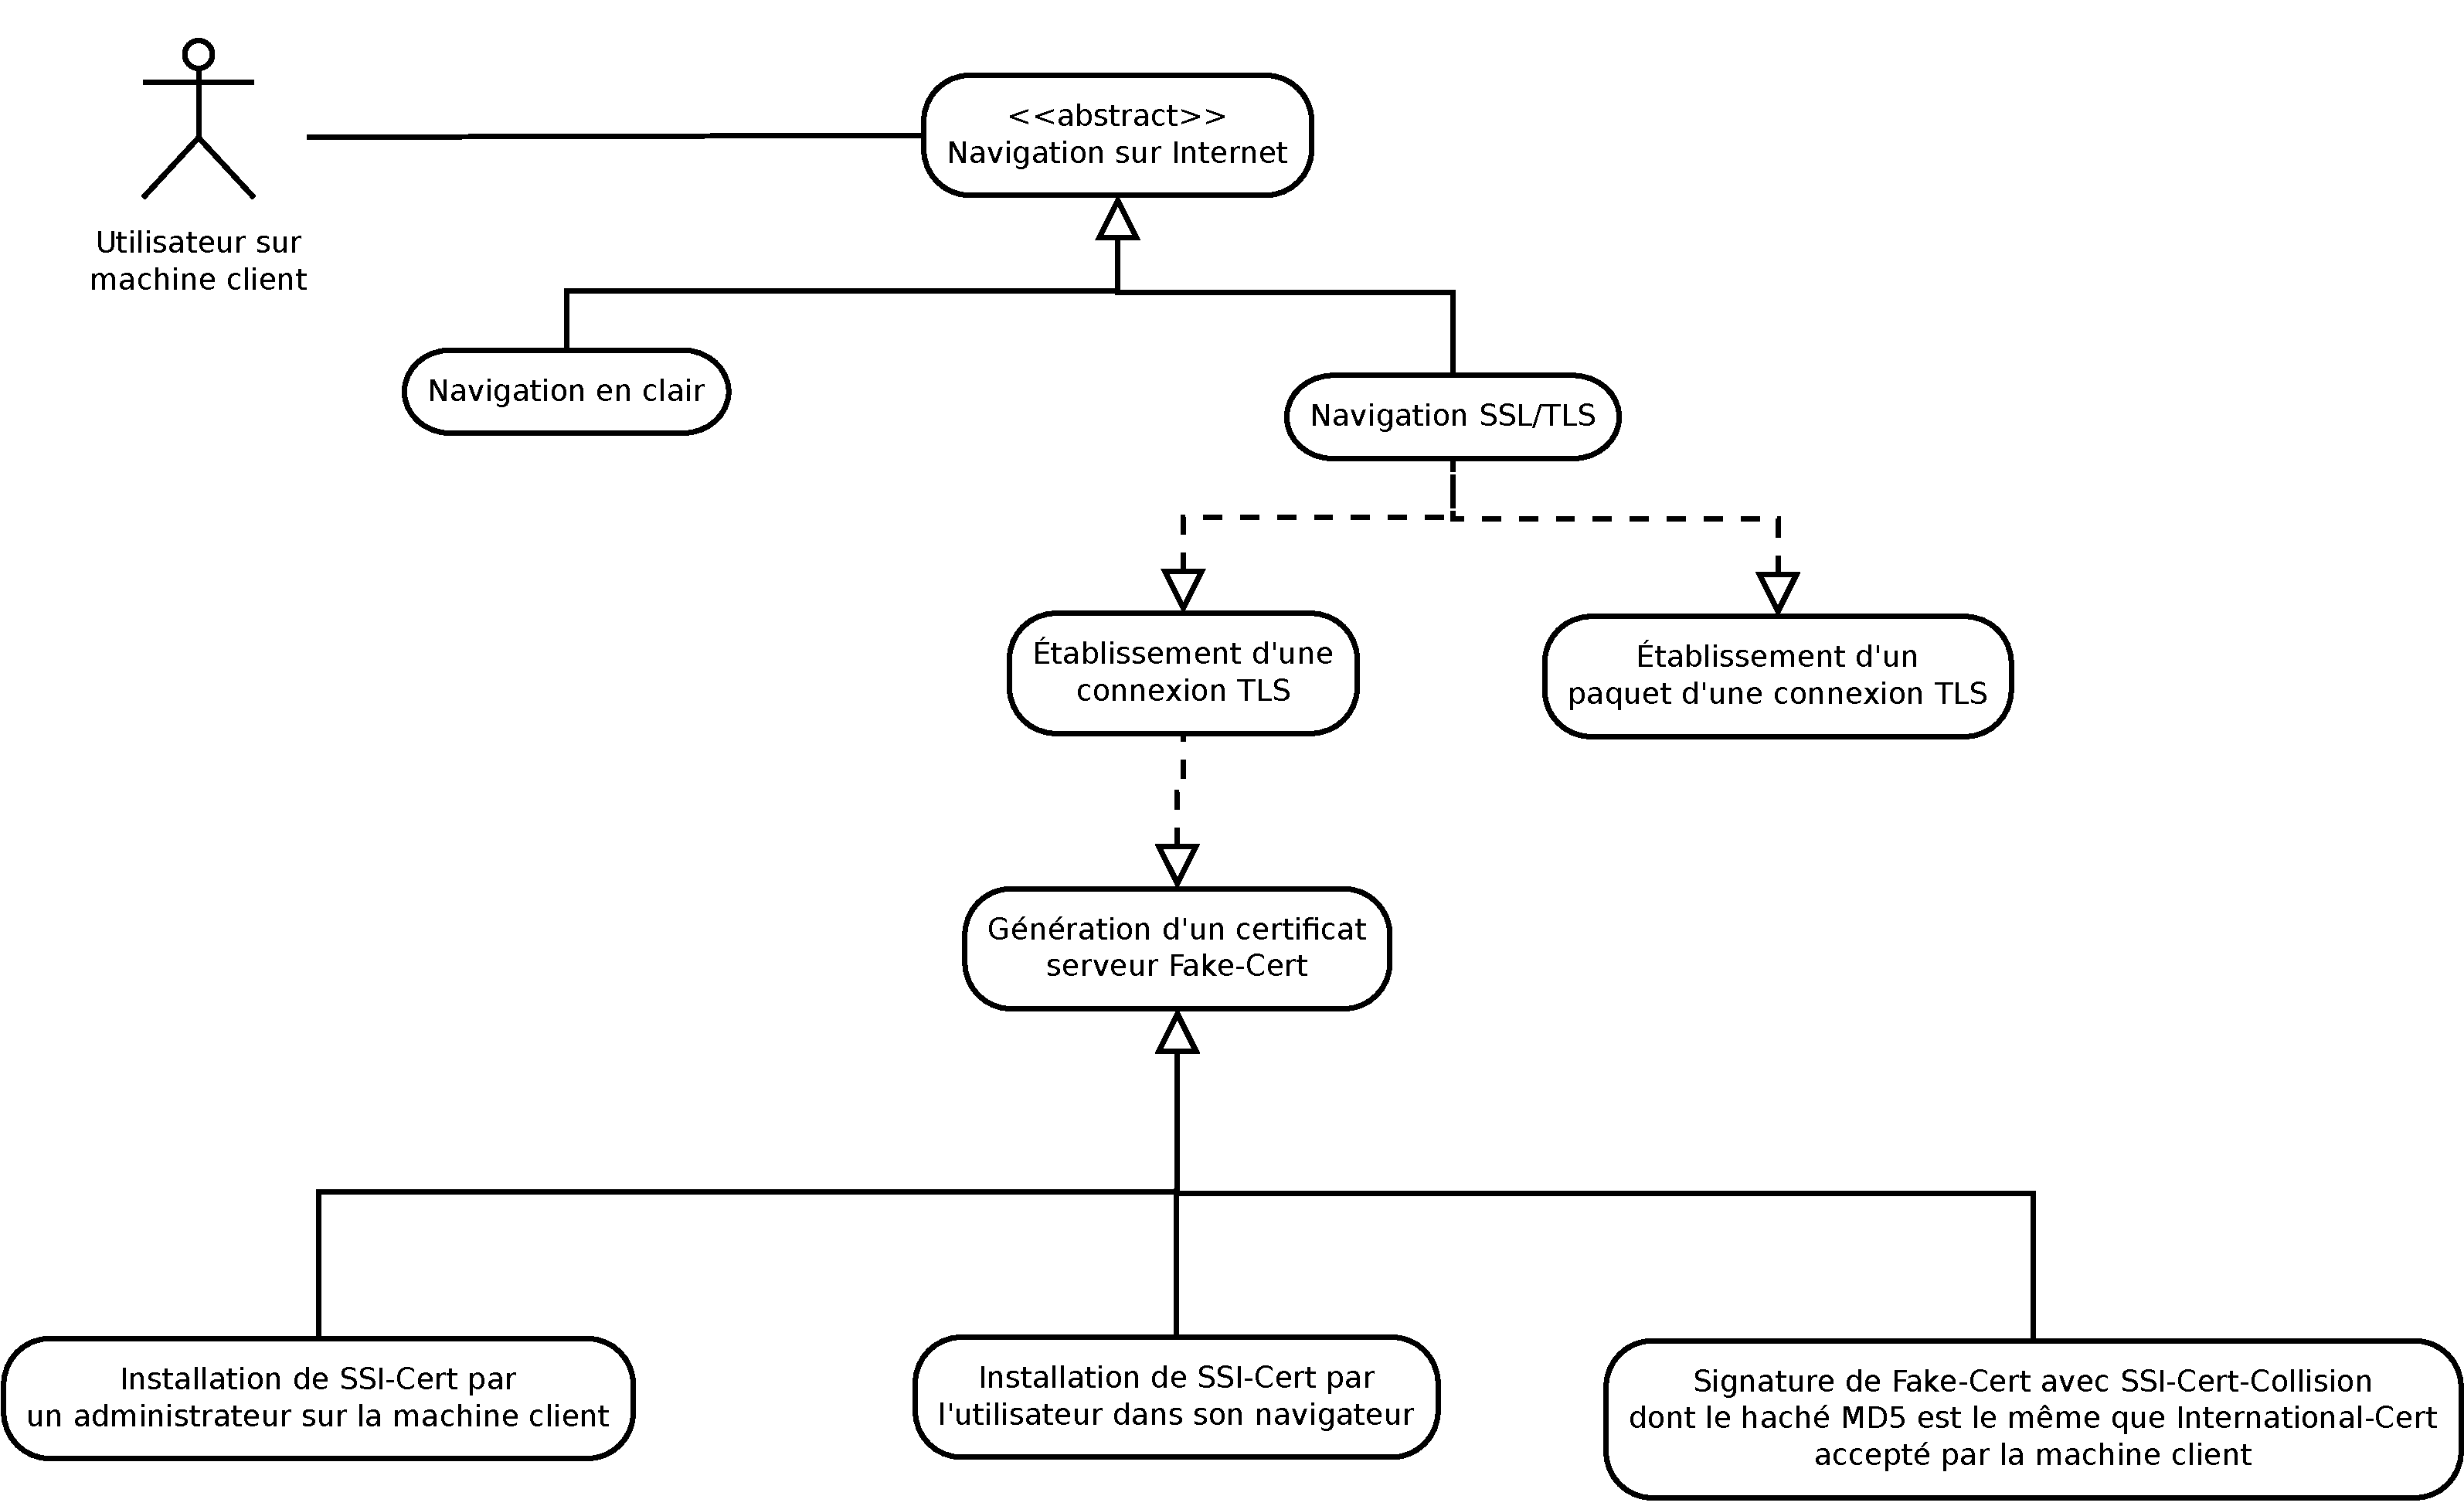
\includegraphics[width=0.8\textwidth]{../../STB/images/cas_utilisation.pdf}

\subsection{Schéma du système}
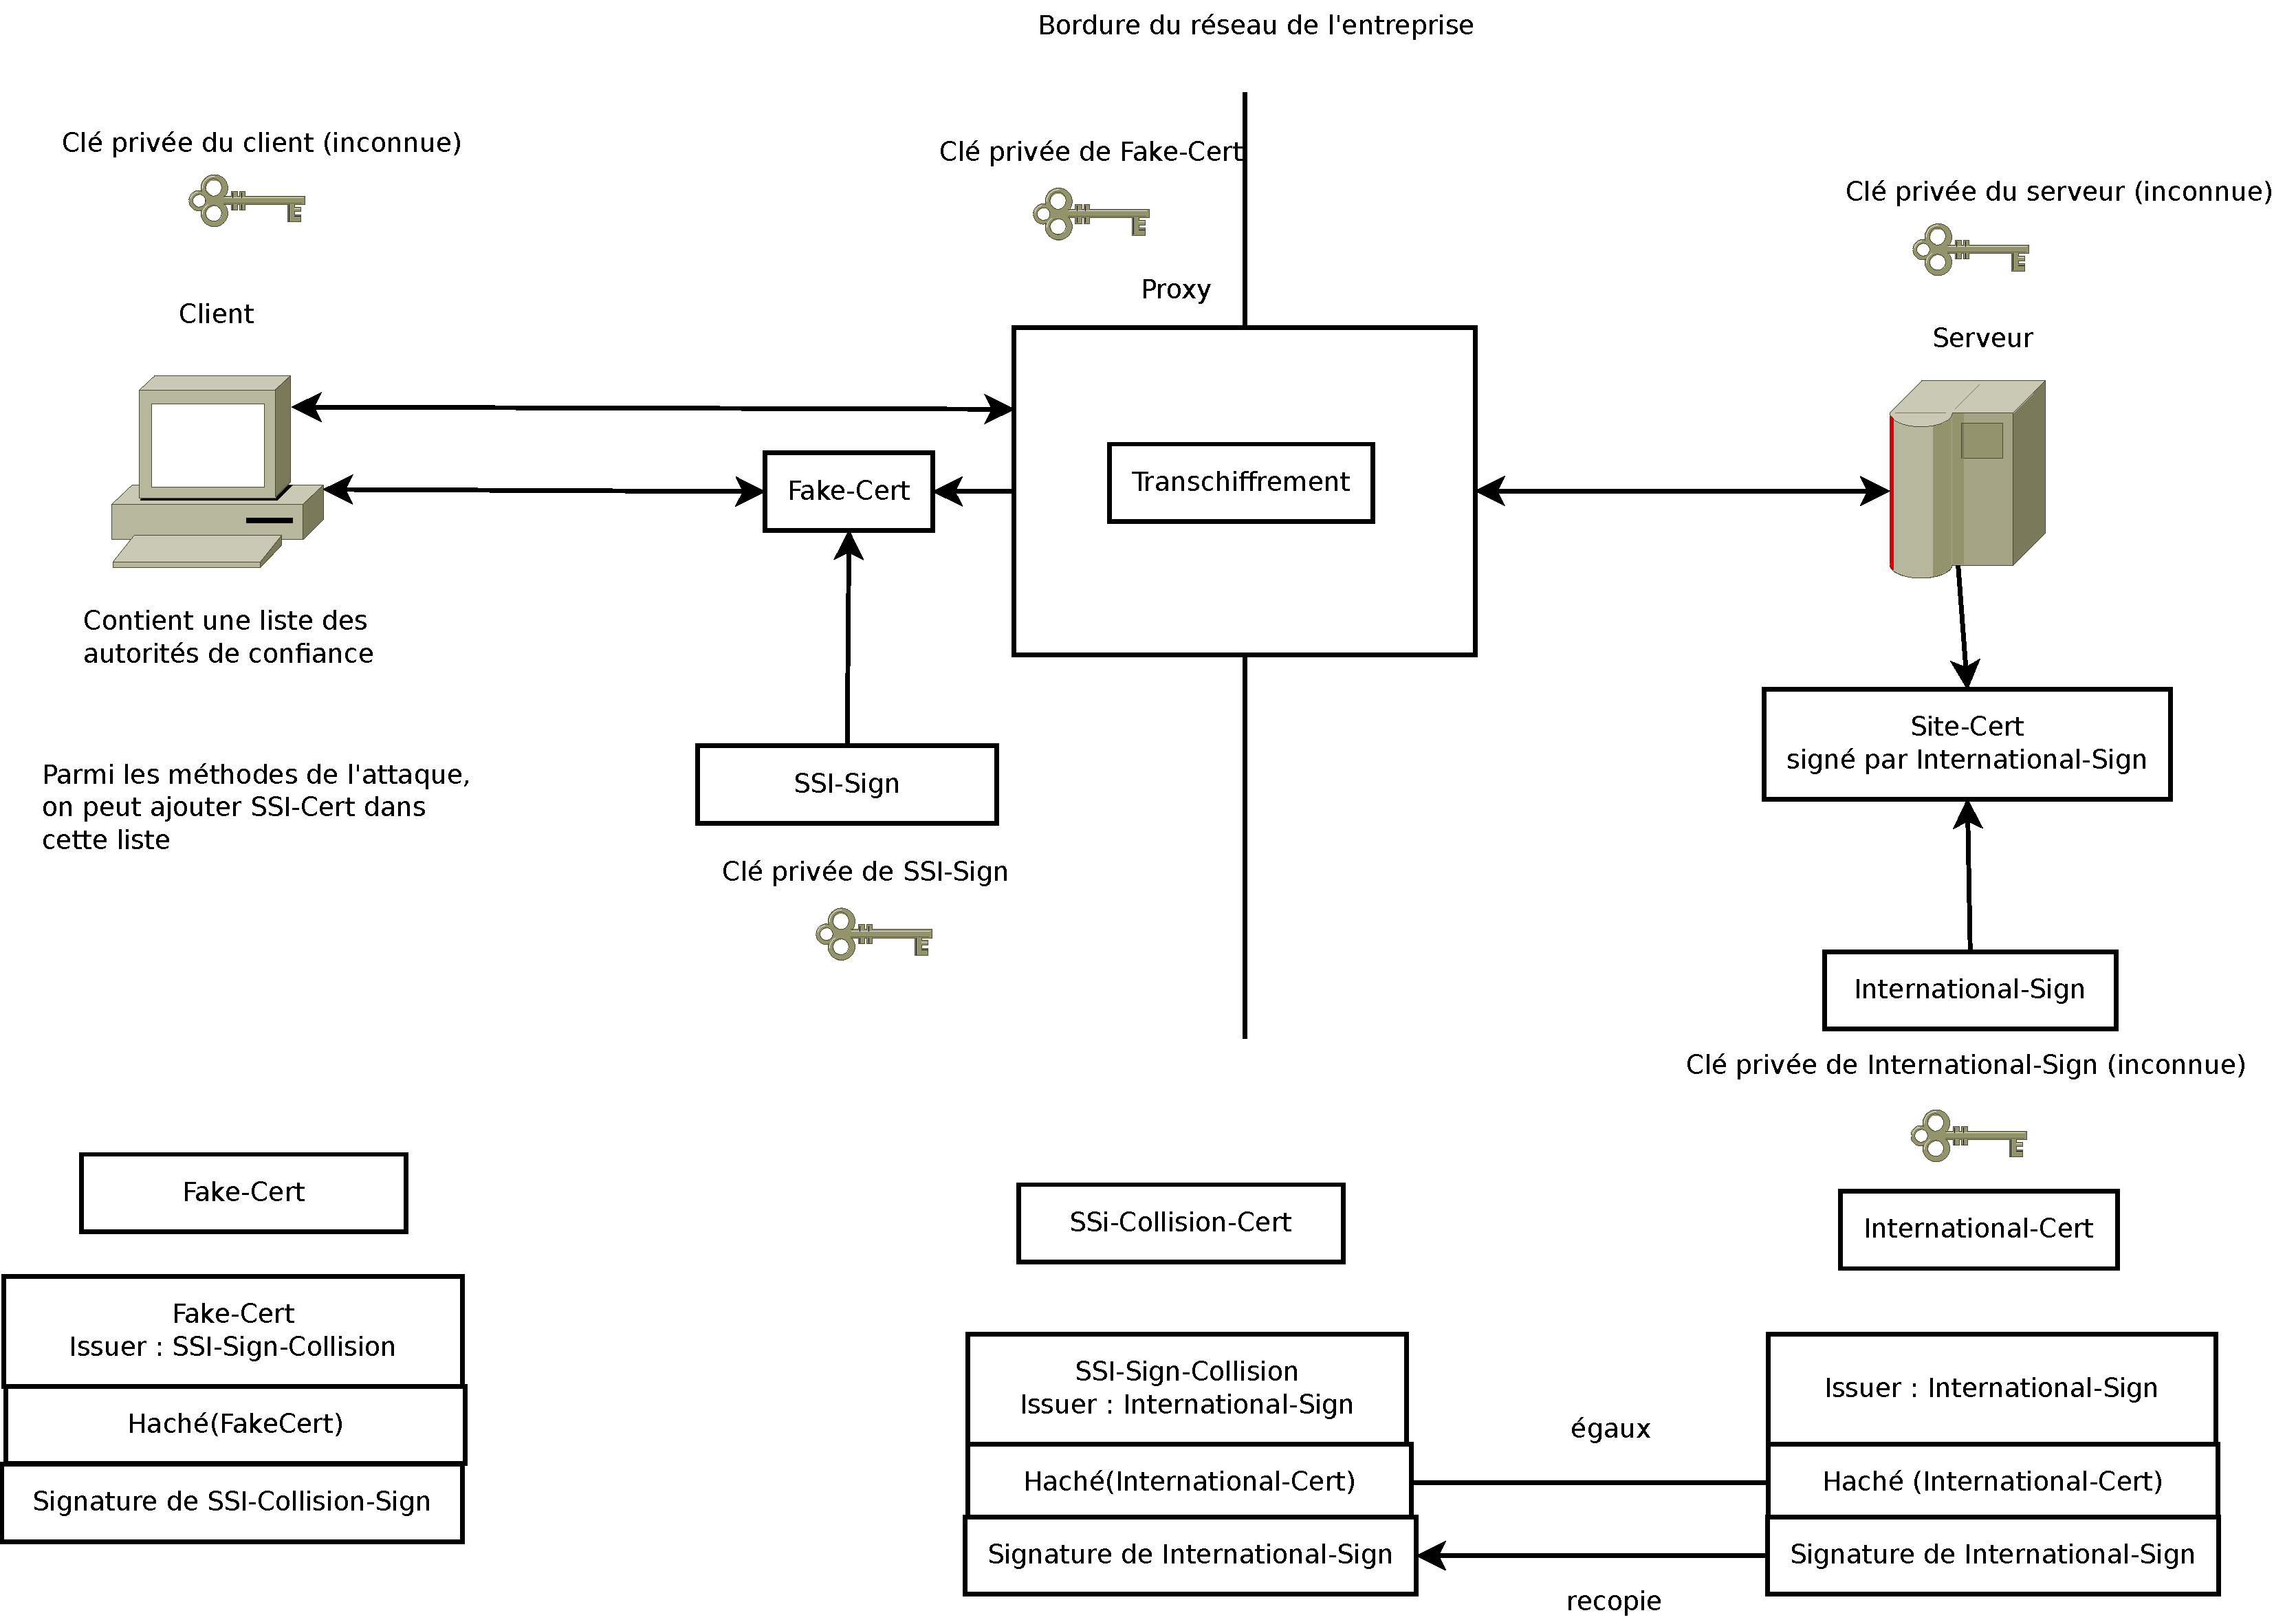
\includegraphics[width=0.8\textwidth]{../../STB/images/schema_autorites.pdf}


\section{Gestion de projet}

\subsection{L'équipe}

Pour mener à bien ce projet, nous sommes une équipe de 5 étudiants.

Nous nous sommes répartis autour des deux parties principales parties du projet.
\begin{itemize}
  \item Un proxy de transchiffrement SSL.
  \item La rechercher de collision sur des certificats de type MD5.

\end{itemize}

\subsection{Présentation des livrables}

Les fonctionnalités finales attendues sont :
\begin{itemize}
\item Une application servant de proxy réalisant du transchiffrement SSL.
\item Un dossier de recherche sur les collisions de certificats de type MD5, ainsi qu'une mise en oeuvre 
par un algorithme de recherche.
\end{itemize}

\subsection{Évolution du planning et des priorités}

Nous avons rencontré des difficultés dans la réalisation du projet.
En accord avec le client, nous avons privilégié la réalisation du programme applicatif de proxy.

\subsection{Gestion des risques}

Nous avons établi une liste des risques qui pouvaient menacer la réussite du projet.

Ces risques ont fait l'objet d'une attention particulière, tout au long du projet.

\chapter{Proxy SSL/TLS}
\section{Analyse}

\subsection{Cibles visées par l'attaque}

\subsection{Protocole TLS}
\subsubsection{Définition}
Le protocole TLS/SSL est un protocole de sécurisation des échanges sur internet. Il fonctionne suivant un mode client/serveur
TLS/SSL assure l'authentification, la confidentialité et l'intégrité.
\subsubsection{Fragmentation}
La fragmentation des blocs d'informations en des "record" TLS/SSL porte sur des données 2\^\ 14 octets ou moins.
\subsubsection{Fonction HMAC}
Pour protéger l'intégrité du message TLS/SSL utilise le code MAC,
le chiffrement utilise une construction HMAC qui est basée sur une fonction de hachage.
\subsubsection{Le protocole "record" TLS/SSL}
\begin{itemize}
\item L'envoi:
TLS/SSL prend les messages à transmettre, fragmente les données en des blocs, compresse les données (optionnel), applique le MAC, chiffre et transmet le résultat. 
\item
La réception:
A la réception, les données sont déchiffrées, vérifiées, décompressées, rassemblées, puis elles sont livrées à des clients de niveau supérieur.
\end{itemize}
le protocole handshake utilise ce genre d'échange de message.
\subsubsection{Le protocole handshake:}

Le protocole handshake est responsable pour la négociation d'une session.
Cette session se compose des éléments suivants:
\begin{itemize}
\item Session identifier: séquences de bit arbitraires choisis par le serveur pour identifier une session active.
\item Peer certificate: ce champ contient le certificat X509v3. 
\item Compression method: l'algorithme utilisé pour compresser les données avant le chiffrement.
\item Cipher spec: spécifie la fonction utilisée pour générer des clés, l'algorithme de chiffrement, l'algorithme MAC et les attributs cryptographiques.
\item Master secret: le secret partagé entre le client et le serveur.
\item Is resumable: un flag qui indique si la session peut être utilisée pour initialiser une nouvelle connexion ou non.\\
\end{itemize}
Le protocole handshake utilise les étapes suivantes:
\begin{itemize}
\item Echanger un message "hello messages" pour se mettre d'accord sur l'algorithme.
\item Echanger des paramètres cryptographiques pour accepter le secret entre le client et le serveur.
\item Echanger les certificats et des informations cryptographiques pour permettre au client et au serveur de s'authentifier. 
\item Générer un secret à partir d'un autre et échange des valeurs aléatoires.
\item Fournir les paramètres de sécurité.
\item Permettre au client et au serveur de vérifier qu'ils ont le même paramètre de sécurité et que le handshake a eu lieu sans altération d'un attaquant.
\end{itemize}
\paragraph{Hello request}
C'est une notification pour que le client initie la négociation d'une connexion.
Le message "Hello request" peut être envoyé à n'importe quel moment.
\paragraph{Client Hello}
Lors de la première connexion du client au serveur, il est nécessaire d'envoyer un "Client hello" comme premier message.
Le client peut aussi envoyer un "Client hello" comme une réponse de "Hello request".
Ce message contient la date, un nonce et les algorithmes disponibles.
\paragraph{Server Hello}
Le serveur va envoyer ce message suite a un "Client hello" si il y a un algorithme commun, sinon il envoie un "Failure alert".
Ce message contient la date, un nonce et l'algorithme choisi.
\paragraph{Server Certificate}
Le serveur envoie son certificat pour s'authentifier auprès du client.
Ce message contient un Site-Cert ainsi que les certificats de la chaîne de certification (Autorité).
\paragraph{Client Certificate Request}
Optionnel, seulement si le serveur veut que le client soit authentifié.
\paragraph{Server Hello Done}
Indique la fin d'envoi du serveur.
\paragraph{Client Certificate}
Si (Client Certificate Request) est émis, alors le client envoie son certificat pour l'authentification client. 
\paragraph{Client Key Exchange}
Paquet chiffré avec la clé publique du serveur qui contient une clé de session générée à partir des deux nonces échangés. Si le serveur est capable de déchiffrer et de répondre, il est authentifié auprès du client.
\paragraph{Client Verify}
Si (Client Certificate Request) est émis, le client devra signer avec sa clé privée un haché des échanges précédents, ce qui l'authentifiera auprès du serveur. 
\paragraph{Change Cipher Spec.}
Précise que tous les paquets envoyés à la suite du "Client Finished" seront chiffrés avec la clé de session échangée et les algorithmes choisis. 
\paragraph{Client Finished}
Informe que le client a fini et contient un haché de la totalité des échanges. 
\paragraph{Change Cipher Spec.}
Précise qu'à partir de maintenant, le serveur va envoyer des paquets chiffrés. 
\paragraph{Server Finished}
Contient un haché de tous les échanges chiffré avec la clé de session et un MAC.

\section{Conception}

\subsection{UML}
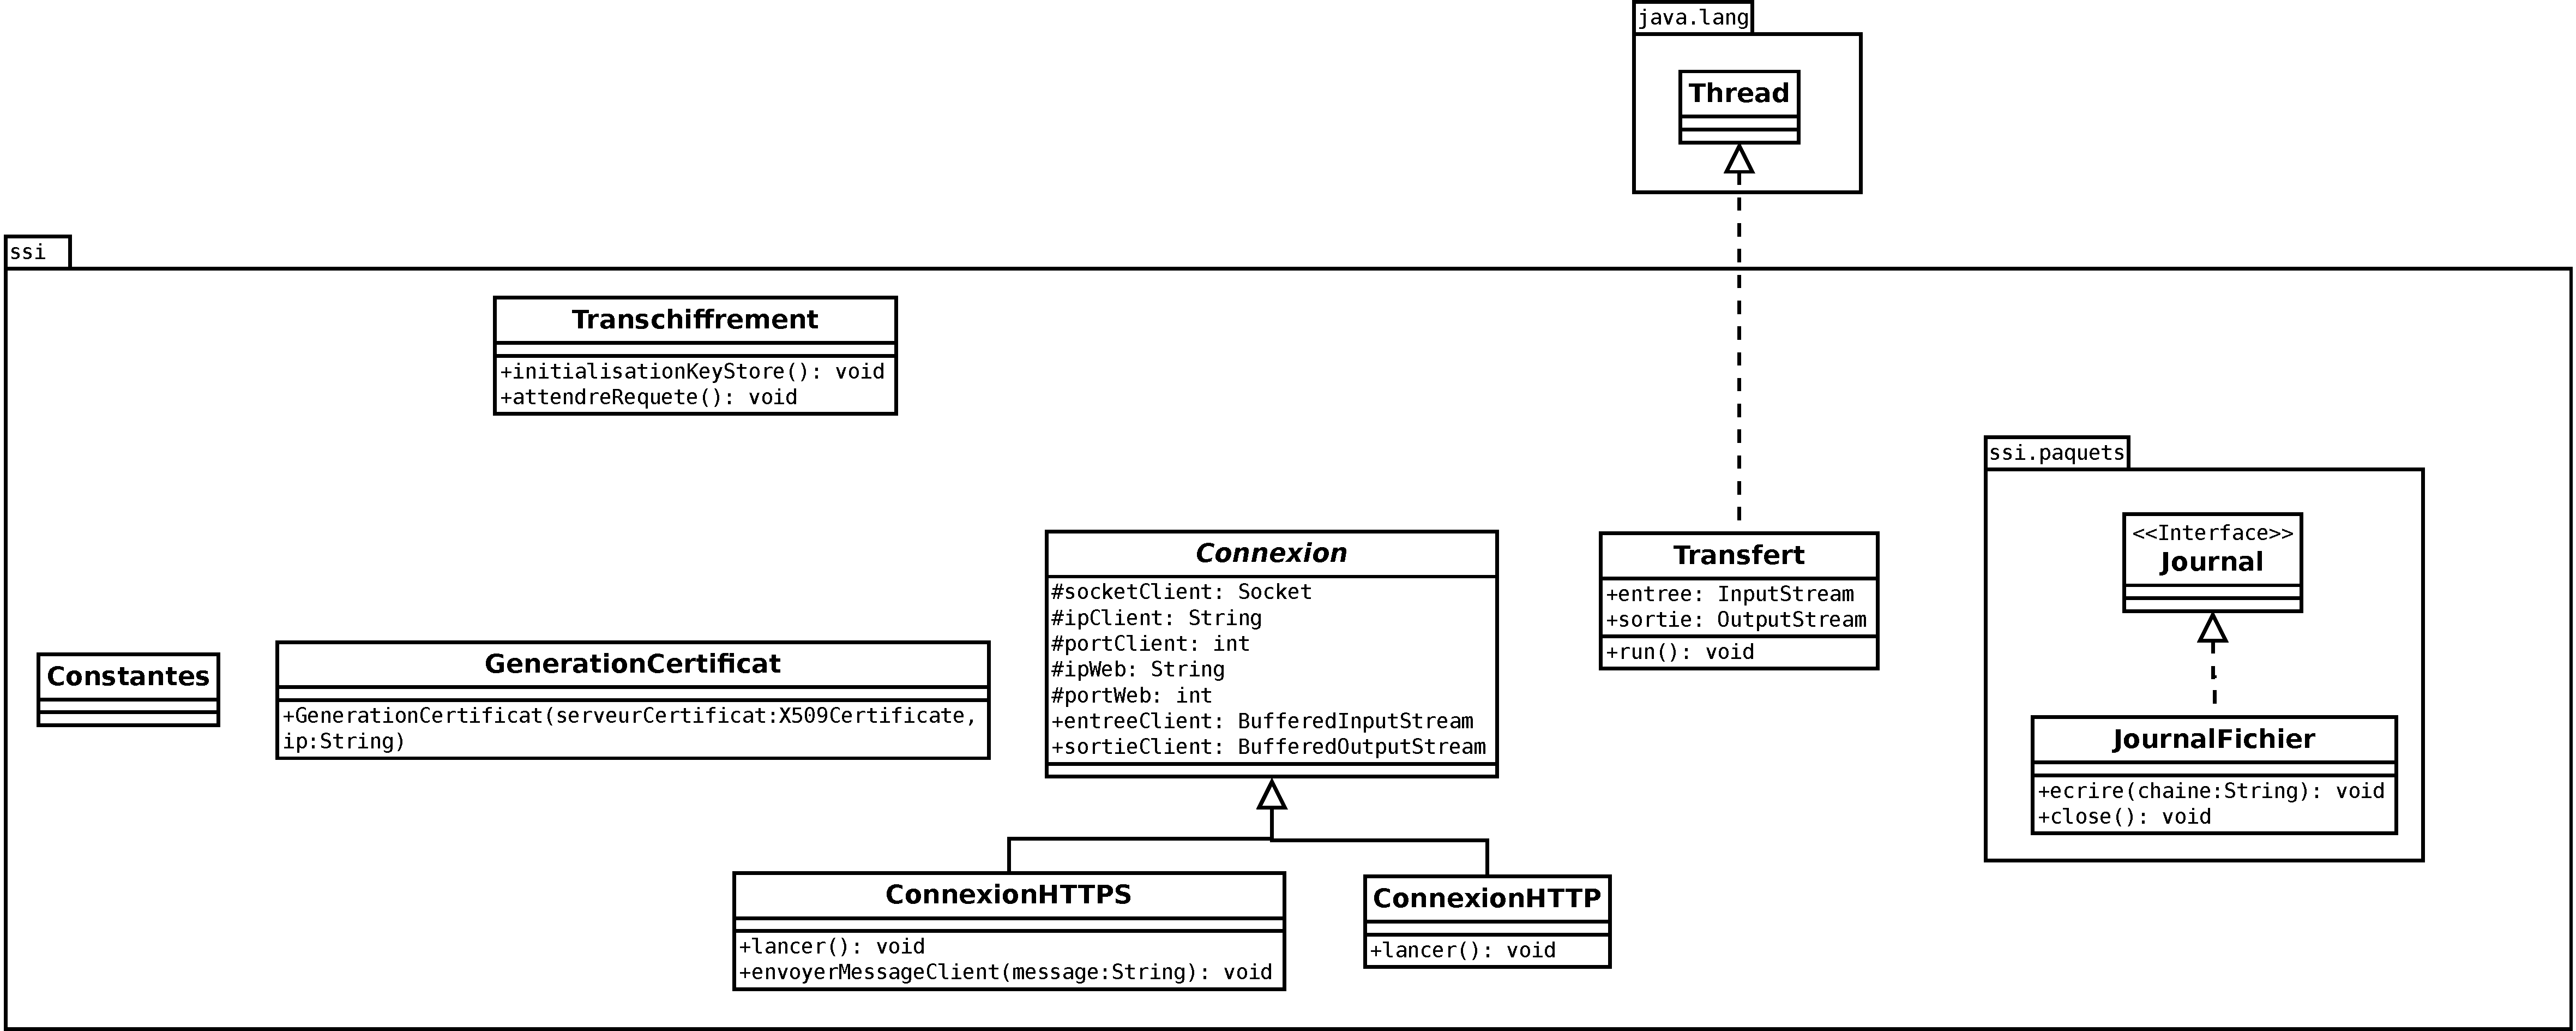
\includegraphics[width=0.8\textwidth]{images/uml.pdf}
~~\\
~~\\
Rôle des différentes classes:
\begin{itemize}
	\item Transchiffrement: classe principale de l'application, elle contient le main et va permettre la création de la socket serveur et la détection du type de connexion entrantes (HTTP ou HTTPS).
	\item GenerationCertificat: cette classe permet de forger un faux certificat en fonction de celui récupéré lors de l'établissement d'une connexion HTTPS.
	\item Transfert: classe permettant la création de threads pour l'échange des données entre les différentes entités (voir schéma partie 2.4.1).
	\item Connexion: une classe abstraite qui permet de mutualiser le code commun entre les connexions HTTP ou HTTPS.
	\item ConnexionHTTP: permet de gérer les connexions HTTP, avec le lancement de deux threads pour l'échange des données grâce a la classe Transfert.
	\item ConnexionHTTPS: permet de gérer les connexions HTTPS, appel de la classe GenerationCertificat pour forger le faux certificat et lancement de deux threads pour l'échange des données grâce a la classe Transfert.
	\item Constantes: cette classe regroupe toutes les valeurs constantes utilisées dans la plupart des classes du projet.
	\item JournalFichier: cette classe permet la création, l'ouverture et le remplissage d'un fichier de avec les logs récupérés lors des échanges de type HTTP et HTTPS.
\end{itemize}

\section{Implémentation}
\subsection{Faire accepter une autorité}
\documentclass[a4paper,11pt,french]{book}
\usepackage[utf8]{inputenc}

\usepackage[T1]{fontenc}
\usepackage[francais]{babel} 
\usepackage[top=2cm, bottom=2cm, left=2cm, right=2cm, includeheadfoot]{geometry} %pour les marges
\usepackage{lmodern}
\usepackage{pict2e}
\usepackage{fancyhdr} % Required for custom headers
\usepackage{lastpage} % Required to determine the last page for the footer
\usepackage{extramarks} % Required for headers and footers
\usepackage{graphicx} % Required to insert images
\usepackage{tabularx, longtable}
\usepackage{color, colortbl}
\usepackage{lscape}
%\usepackage[hidelinks]{hyperref}
\usepackage{longtable}
\usepackage{multirow}
\usepackage{rotating}
\usepackage{gensymb}

\usepackage{algorithm}
\usepackage{algorithmic}


\linespread{1.1} % Line spacing

% Set up the header and footer
\pagestyle{fancy}
\lhead{\textbf{\hmwkClass -- \hmwkSubject \\ \hmwkTitle \\ \hmwkDocName}} % Top left header
\rhead{
\includegraphics[width=10em]{logo_univ.png}}
\lfoot{\lastxmark} % Bottom left footer
\cfoot{} % Bottom center footer
\rfoot{Page\ \thepage\ / \pageref{LastPage}} % Bottom right footer
\renewcommand\headrulewidth{0.4pt} % Size of the header rule
\renewcommand\footrulewidth{0.4pt} % Size of the footer rule

\setlength{\headheight}{40pt}

\newcommand{\hmwkTitle}{\'Etude sur l'installation/acceptation d'une autorité de certification} % Assignment title
\newcommand{\hmwkClass}{Master 2 SSI } % Course/class
\newcommand{\hmwkAuthorName}{Julien BOURDON} % Your name
\newcommand{\hmwkSubject}{Recherche} % Subject
\newcommand{\hmwkDocName}{} % Document name

\newcommand{\version}{1.0} % Document version
\newcommand{\docDate}{28 novembre 2013} % Document date
\newcommand{\checked}{} % Checker name
\newcommand{\approved}{} % Approver name

\makeatletter
\newcommand{\resettranslate}{\let\translate\@firstofone}
\makeatother

\definecolor{gris}{rgb}{0.95, 0.95, 0.95}

\title{
\vspace{2in}
\textmd{\textbf{\hmwkClass :\ \hmwkTitle}}\\
\normalsize\vspace{0.1in}\small{Due\ on\ \hmwkDueDate}\\
\vspace{0.1in}\large{\textit{\hmwkClassInstructor\ \hmwkClassTime}}
\vspace{3in}
}

\author{\hmwkAuthorName}
\date{} % Insert date here if you want it to appear below your name


\usepackage{amsmath}
\begin{document}
\newcount\startdate
\newcount\daynum
%\pgfcalendardatetojulian{2013-01-021}{\startdate}
\pagestyle{fancy}

\vspace*{5cm}
\begin{center}\textbf{\Huge{\hmwkDocName}}\end{center}
\vspace*{4.5cm}
	

\fcolorbox{black}{gris}{
\begin{minipage}{15cm}
\begin{tabularx}{10cm}{lXl}
	\bfseries{Version} & & \version\\
	& & \\
	\bfseries{Date} & & \docDate\\
	& & \\
	\bfseries{Rédigé par} & & \hmwkAuthorName \\
	& & \\
	\bfseries{Relu par} & & \checked \\
	& & \\
	\bfseries{Approuvé par} & & \approved \\
	& & \\
\end{tabularx}
\end{minipage}
}

\newpage

%Tableau de mises à jour
\vspace*{1cm}
\begin{center}
\textbf{\huge{MISES À JOUR}}\\
\vspace*{3cm}
	\begin{tabularx}{16cm}{|c|c|X|}
	\hline
	\bfseries{Version} & \bfseries{Date} & \bfseries{Modifications réalisées}\\
	\hline
	1.0 & 28/11/2013 & Création\\
	\hline
	& & \\
	\hline
	\end{tabularx}
\end{center}

%La table des matières
\clearpage
\tableofcontents
\clearpage

\section{Objet}

De nos jours, nous avons besoin d'authentifier les sites auxquels on veut accéder pour être sur que les données cruciales que nous manipulons ne tombent pas en de mauvaises mains. Pour ce faire, on utilise des certificats signés par des autorités en qui on peut avoir confiance.
Ces autorités sont répertoriées dans nos machines et plus précisément dans nos navigateurs par le biais de certificats d'autorité.
Nous allons maintenant voir comment on peut faire accepter l'installation d'une nouvelle autorité sur sa machine en quelques clics.


\section{Installation par un administrateur mal intentionné}
Nous prenons, ici, le cas d'un administrateur ayant un accès à tous les ordinateurs d'une entreprise.
Cette personne veut faire accepter une autorité de certification dont il est le propriétaire pour pouvoir lire tous les paquets qui transitent et surtout les chiffrés.
Nous allons expliquer comment faire pour les principaux navigateurs utilisés sous linux.
Voilà un tableau comparatif des pourcentages d'utilisation des navigateurs : 

Moyenne générale (Décembre 2013) :
\begin{itemize}
\item{Chrome} 		34,73\%
\item{Internet Explorer}		 22,89\%
\item{Firefox} 		18,25\%
\item{Safari} 		16,19\%
\item{Opera}	 		1,57\%	
\item{Autres} 		6,38\%
\end{itemize}	

Nous allons donc privilégier Firefox et Chrome.
\newpage
\subsection{Mozilla Firefox}

Tout d'abord, l'administrateur ouvre Firefox puis clique sur Edit > Preferences.

\includegraphics[width=\textwidth]{images/OngletPref.png}
\newpage
Ensuite, il choisit Advanced > Certificates > View Certificates.

\includegraphics[width=\textwidth]{images/OngletCert.png}
\newpage
Il va ensuite dans Authorities > Import.

\includegraphics[width=\textwidth]{images/OngletCA.png}
\newpage
Il choisit ensuite le certificat de l'autorité qu'il veut installer puis valide.

\includegraphics[width=\textwidth]{images/OngletImport.png}
\newpage
Une fenêtre s'ouvre et propose de faire confiance à cette autorité pour 3 types de Certificats. L'administrateur coche les 3 cases pour que son autorité soit reconnue valide sur tous les types puis clique sur ok.

\includegraphics[width=\textwidth]{images/OngletConfirm.png} 


Voilà, l'autorité est installée et tous les certificats signés par cette autorité seront reconnus comme valides.
\newpage
\subsection{Chrome}

La démarche est très similaire à celle de firefox.

Tout d'abord, l'administrateur va dans Modifier > Préférences

\includegraphics[width=\textwidth]{images/ChromePref.png} 
\newpage

Puis il clique sur Afficher les paramètres avancés.

\includegraphics[width=\textwidth]{images/ChromeAvance.png} 
\newpage

Ensuite, dans la partie HTTPS/SSL, il clique sur Gérer les certificats

\includegraphics[width=\textwidth]{images/ChromeCert.png} 
\newpage

Il se déplace dans Autorités et clique sur Importer

\includegraphics[width=\textwidth]{images/ChromeCA.png} 
\newpage

Il choisit le certificat de l'autorité et valide.

\includegraphics[width=\textwidth]{images/ChromeImport.png} 
\newpage

Enfin, il coche les 3 cases et clique sur ok pour finaliser l'installation de l'autorité.

\includegraphics[width=\textwidth]{images/ChromeValide.png} 
\newpage

\section{Forcer l'acceptation de l'autorité par un client}
Dans cette section, nous forçons l'utilisateur a accepter notre autorité de certification. Si il ne l'a pas, il ne pourra pas naviguer sur internet.
Nous proposons donc un lien pour récupérer le certificat d'autorité sur lequel il faut cliquer.

\includegraphics[width=\textwidth]{images/Page.png} 
\newpage

Ensuite, la fenêtre de validation s'ouvre et le client doit cocher les cases puis valider.

\includegraphics[width=\textwidth]{images/Cert.png} 
\newpage

A ce stade, l'autorité est installée et si le client veut retenter de l'installer, un message le prévient qu'il a déjà fini l'installation.

\includegraphics[width=\textwidth]{images/Alerte.png}

On peut voir qu'en seulement quelques clics, l'utilisateur installe une autorité dont il ne connaît rien et qui peut être utilisée pour déchiffrer toutes ses informations personnelles. 
\newpage
\end{document}

\subsection{Threads}

Une fois une connexion établie, nous avons au niveau du proxy deux Sockets (bi-directionnelles), une vers le serveur, et une vers le client.

Chaque Socket est composée de deux Stream (uni-directionnels), un en entrée et l'autre en sortie.

Jusqu'à ce que la connexion soit interrompue, nous devons faire transiter les paquets, de l'entrée vers la sortie, et réciproquement pour le deuxième stream de la socket.

Pour ce faire, pour chaque nous lançons un objet de type Transfert dans un nouveau Thread.

Cela permet de continuer les traitements en parallèle, sans que l'application soit bloquée par un read.

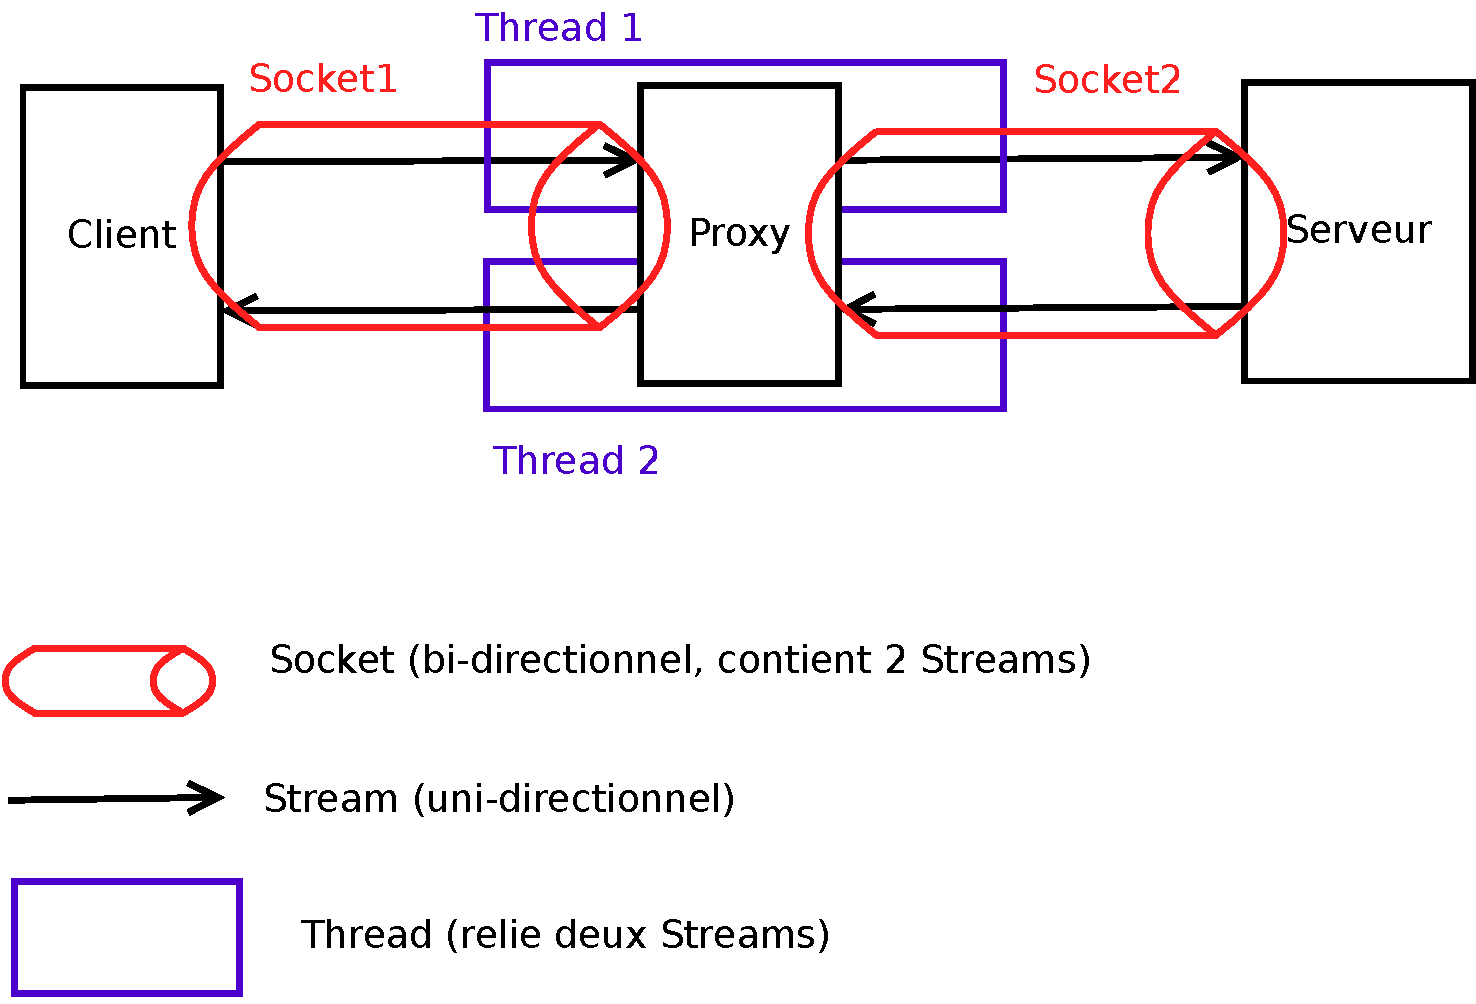
\includegraphics[width=0.8\textwidth]{images/thread.pdf}

\subsection{Sockets}
Pour ce projet, nous devons faire communiquer les différents composants du projet ensemble. Ces composants sont :
\begin{itemize}
\item Le navigateur du client.
\item Le proxy.
\item Le serveur Web.
\end{itemize}

Suite à la phase d'analyse, nous avons décidé d'utiliser les sockets, qui sont implémentées en Java.
=======
Suite à la phase d'analyse, nous avons décidé d'utiliser les sockets, qui sont implémentées en Java 
et mise en place sur le proxy. Le proxy a besoin de mettre en place deux 
connexions distinctes, une avec le client (navigateur web) et une avec le serveur web. Il faut donc utiliser 
deux types de connexions:
\begin{itemize}
  \item Serveur, pour établir une connexion avec le client.
  \item Client, pour établir une connexion avec le serveur web distant
\end{itemize}
Il existe deux grand types de socket dans la librairie Java, Socket et SSLSocket 
avec leur dérivées ServerSocket et SSLServerSocket.
~~\\
Lors d'une connexion HTTPS, l'utilisation des sockets SSL permet directement de 
faire le chiffrement et le déchiffrement des données. Les données échangées sont 
uniquement chiffrées dans les sockets SSL, en entrée et sortie les données sont 
lisibles en clair sur le proxy.
Pour chiffrer et déchiffrer avec les bons algorithmes, on utilise la liste des 
algorithmes disponibles sur le serveur web et prenant le premier algorithme 
commun entre ceux du serveur et ceux disponible par les sockets SSL Java.
La méthode utilisée pour trouver ces algorithme est getCipherSuite().
~~\\
La création de sockets SSL demande au préalable la création d'un contexte SSL. 
Ce contexte se créer en utilisant le certificat du serveur, ou le certificat 
généré par le proxy. Une fois le contexte mis en place on peut créer les sockets 
SSL, et donc mettre en place le tunnel SSL. Les sockets seront automatiquement configurées pour échanger des données 
uniquement avec le serveur web qui détient le certificat qui a permis la 
création du contexte.
Sans contexte, la création de sockets SSL ne permet pas d'échanger des données 
dans un tunnel SSL.

Chacun des deux types de sockets sont implémentées en en mode simple (Socket) et 
en mode SSL (SSLSocket) suivant le type de connexion demandée par le client. A 
noter qu'il est obligaoire de créer des sockets simple même en cas de connexion 
HTTPS.

Création des sockets pour la connexion HTTP sur chacune des deux parties du proxy:
\begin{itemize}
  \item Serveur: on commence par créer une socket de type ServerSocket qui va 
  être en écoute et attendre la connexion d'un client avec la méthode accept(). 
  Cette méthode est blocante tant qu'il n'y a pas d'initialisation de connexion 
  par un client. Dès que la ServerSocket reçoit une demande de connexion
  elle va créer une socket de type Socket. Ces deux sockets seront utilisées pour la communication entre le client (navigateur web) et le proxy.
  Quelque soit le type de la requête du client (HTTP ou HTTPS), la 
  création de ces deux sockets est obligatoire.
  
  \item Client: après la création de la connexion Serveur, on récupère 
  l'adresse IP et le port dans la requête du client pour faire une demande de 
  connexion auprès du serveur web, ce qui entraîne la création d'une socket de 
  type Socket. Cette socket sera utilisée uniquement pour la communication entre 
  le proxy et le serveur web distant. 
\end{itemize}

Création des sockets pour la connexion HTTPS sur chacune des deux parties du proxy:
\begin{itemize}
  \item Serveur: la première partie est identique qu'en HTTP. Pour la deuxième 
  partie on récupère le certificat du serveur pour forger notre propre 
  certificat serveur basé sur celui du serveur web. Ensuite on créer un contexte 
  avec ce nouveau certificat pour créer une SSLServerSocket et une SSLSocket 
  pour léchange des données dans le tunnel SSL entre le navigateur web et le 
  proxy.
  
  \item Client: on récupère l'adresse IP et le port dans la requête du client 
  pour aller chercher le certificat du serveur web. A partir de ce certificat on 
  créer un contexte SSL pour pourvoir générer la sockets SSL et mettre en place 
  le tunnel SSL entre le proxy et le serveur web distant.
\end{itemize}

\subsection{Keystore}
\documentclass[a4paper,11pt,french]{article}
\usepackage[utf8]{inputenc}

\usepackage[T1]{fontenc}
\usepackage[francais]{babel} 
\usepackage[top=2cm, bottom=2cm, left=2cm, right=2cm, includeheadfoot]{geometry} %pour les marges
\usepackage{lmodern}
\usepackage{pict2e}
\usepackage{fancyhdr} % Required for custom headers
\usepackage{lastpage} % Required to determine the last page for the footer
\usepackage{extramarks} % Required for headers and footers
\usepackage{graphicx} % Required to insert images
\usepackage{tabularx, longtable}
\usepackage{color, colortbl}
\usepackage{lscape}
%\usepackage[hidelinks]{hyperref}
\usepackage{longtable}
\usepackage{multirow}
\usepackage{rotating}
\usepackage{gensymb}
\usepackage{soulutf8}

\linespread{1.1} % Line spacing

% Set up the header and footer
\pagestyle{fancy}
\lhead{\textbf{\hmwkClass -- \hmwkSubject \\ \hmwkTitle \\ \hmwkDocName}} % Top left header
\rhead{
\includegraphics[width=10em]{../../images/logo_univ.png}}
\lfoot{\lastxmark} % Bottom left footer
\cfoot{} % Bottom center footer
\rfoot{Page\ \thepage\ / \pageref{LastPage}} % Bottom right footer
\renewcommand\headrulewidth{0.4pt} % Size of the header rule
\renewcommand\footrulewidth{0.4pt} % Size of the footer rule

\setlength{\headheight}{40pt}

\newcommand{\hmwkTitle}{Transchiffrement} % Assignment title
\newcommand{\hmwkClass}{Master 2 SSI } % Course/class
\newcommand{\hmwkAuthorName}{Émile GÉNÉRAT} % Your name
\newcommand{\hmwkSubject}{Conduite de projet} % Subject
\newcommand{\hmwkDocName}{Spécification Technique du Besoin} % Document name

\newcommand{\version}{1.0} % Document version
\newcommand{\docDate}{} % Document date
\newcommand{\checked}{Jean-Baptiste SOUCHAL} % Checker name
\newcommand{\approved}{} % Approver name

\makeatletter
\newcommand{\resettranslate}{\let\translate\@firstofone}
\makeatother

\definecolor{gris}{rgb}{0.95, 0.95, 0.95}

\title{
\vspace{2in}
\textmd{\textbf{\hmwkClass :\ \hmwkTitle}}\\
\normalsize\vspace{0.1in}\small{Due\ on\ \hmwkDueDate}\\
\vspace{0.1in}\large{\textit{\hmwkClassInstructor\ \hmwkClassTime}}
\vspace{3in}
}

\author{\hmwkAuthorName}
\date{} % Insert date here if you want it to appear below your name


\usepackage{amsmath}
\begin{document}
\newcount\startdate
\newcount\daynum
%\pgfcalendardatetojulian{2013-01-021}{\startdate}
\pagestyle{fancy}

\vspace*{5cm}
\begin{center}\textbf{\Huge{\hmwkDocName}}\end{center}
\vspace*{4.5cm}
	

\fcolorbox{black}{gris}{
\begin{minipage}{15cm}
\begin{tabularx}{10cm}{lXl}
	\bfseries{Version} & & \version\\
	& & \\
	\bfseries{Date} & & \docDate\\
	& & \\
	\bfseries{Rédigé par} & & \hmwkAuthorName \\
	& & \\
	\bfseries{Relu par} & & \checked \\
	& & \\
	\bfseries{Approuvé par} & & \approved \\
	& & \\
\end{tabularx}
\end{minipage}
}

\newpage

%Tableau de mises à jour
\vspace*{1cm}
\begin{center}
\textbf{\huge{Versions}}\\
\vspace*{3cm}
	\begin{tabularx}{16cm}{|c|c|X|}
	\hline
	\bfseries{Version} & \bfseries{Date} & \bfseries{Modifications réalisées}\\
	\hline
	1.0 &  & Création\\
	\hline
	\end{tabularx}
\end{center}

%La table des matières
\clearpage
\tableofcontents
\clearpage


javax.net.ssl.keyStore- Location of the Java keystore file containing an application process's own certificate and private key. On Windows, the specified pathname must use forward slashes, /, in place of backslashes.

javax.net.ssl.keyStorePassword - Password to access the private key from the keystore file specified by javax.net.ssl.keyStore. This password is used twice: To unlock the keystore file (store password), and To decrypt the private key stored in the keystore (key password).

javax.net.ssl.trustStore - Location of the Java keystore file containing the collection of CA certificates trusted by this application process (trust store). On Windows, the specified pathname must use forward slashes, /, in place of backslashes.

If a trust store location is not specified using this property, the SunJSSE implementation searches for and uses a keystore file in the following locations (in order):

\begin{verbatim}
$JAVA_HOME/lib/security/jssecacerts
$JAVA_HOME/lib/security/cacerts
\end{verbatim}
javax.net.ssl.trustStorePassword - Password to unlock the keystore file (store password) specified by javax.net.ssl.trustStore.

javax.net.ssl.trustStoreType - (Optional) For Java keystore file format, this property has the value jks (or JKS). You do not normally specify this property, because its default value is already jks. javax.net.debug To switch on logging for the SSL/TLS layer, set this property to ssl.



A keystore contains private keys, and the certificates with their corresponding public keys.

A truststore contains certificates from other parties that you expect to communicate with, or from Certificate Authorities that you trust to identify other parties.


A keystore contains a private key. You only need this if you are a server, or if the server requires client authentication.

A truststore contains CA certifcates to trust. If your server’s certificate is signed by a recognized CA, the default truststore that ships with the JRE will already trust it (because it already trusts trustworthy CAs), so you don’t need to build your own, or to add anything to the one from the JRE.







In SSL handshake purpose of trustStore is to verify credentials and purpose of keyStore is to provide credential.

keyStore in Java stores private key and certificates corresponding to there public keys and require if you are SSL Server or SSL requires client authentication.

TrustStore stores certificates from third party, your Java application communicate or certificates signed by CA(certificate authorities like Verisign, Thawte, Geotrust or GoDaddy) which can be used to identify third party.

TrustManager determines whether remote connection should be trusted or not i.e. whether remote party is who it claims to and KeyManager decides which authentication credentials should be sent to the remote host for authentication during SSL handshake.

If you are an SSL Server you will use private key during key exchange algorithm and send certificates corresponding to your public keys to client, this certificate is acquired from keyStore. On SSL client side, if its written in Java, it will use certificates stored in trustStore to verify identity of Server. SSL certificates are most commonly comes as .cer file which is added into keyStore or trustStore by using any key management utility e.g. keytool.


\end{document}

\subsection{Journalisation des échanges}
Un des objectif du proxy de transchiffrement est de pouvoir enregistrer tous les 
échanges entre un client et un serveur lors de leur communication. Dans ce but nous
avons réalisé une classe qui nous permet de stocker dans un fichier tout le trafic qui traverse le proxy.

Ensuite, nous avons développé une seconde méthode, pour chercher un éventuel champ password
dans un formulaire POST, ou passé avec GET. Même si en théorie le mot de passe ne doit jamais
être passé dans l'adresse, il existe toujours des développeurs peu précautionneux.
\section{Abstract}
\subsection{Authentification client}

L'authentification client sur un site web avec l'utilisation de certificats permet de créer une authentification forte.
Ce type d'authentification est beaucoup plus sûr qu'une authentification par 
login et mot de passe, trop facilement trouvable par un attaquant.

Cependant, il est rare qu'un site web sécurisé avec HTTPS utilise de l'authentification 
client. Pour gérer une authentification client, les serveurs doivent être configurés d'une certaine manière. 
Pour exemple le site des impôts Français a essayer de mettre en place ce 
type d'authentification mais cela c'est révélé être un échec dû à la difficulté 
apparente pour une majeur partie des utilisateurs.

Dans le cadre de notre projet, l'utilisation d'une authentification client entre le proxy et le serveur web n'est 
pas réalisable du fait que nous ne gérons pas les serveurs des sites web, et il 
est impossible d'imposer à un site une authentification client alors qu'il 
n'implémente pas cette méthode.

D'autre part si le site web demandé par un client demande l'authentification de 
ce dernier, elle ne sera pas possible à implémentée. Un certificat client est 
généré et signé par l'AC du serveur, or le proxy établit une connexion SSL avec 
le client en utilisant ca propre AC, et ne pourra donc pas reconnaitre le 
certificat du client comme valide, lors de la création du contexte SSL avec le client. 



\section{Tests}

\chapter{Recherche de collision sur des certificats hachés en MD5}

\chapter{Synthèse}

\chapter{Annexes}
\subsection{Mozilla Firefox}

Tout d'abord, l'administrateur ouvre Firefox puis clique sur Edit > Preferences.

\includegraphics[width=\textwidth]{images_autorites/OngletPref.png}
\newpage
Ensuite, il choisit Advanced > Certificates > View Certificates.

\includegraphics[width=\textwidth]{images_autorites/OngletCert.png}
\newpage
Il va ensuite dans Authorities > Import.

\includegraphics[width=\textwidth]{images_autorites/OngletCA.png}
\newpage
Il choisit ensuite le certificat de l'autorité qu'il veut installer puis valide.

\includegraphics[width=\textwidth]{images_autorites/OngletImport.png}
\newpage
Une fenêtre s'ouvre et propose de faire confiance à cette autorité pour 3 types de Certificats. L'administrateur coche les 3 cases pour que son autorité soit reconnue valide sur tous les types puis clique sur ok.

\includegraphics[width=\textwidth]{images_autorites/OngletConfirm.png} 


Voilà, l'autorité est installée et tous les certificats signés par cette autorité seront reconnus comme valides.
\newpage
\subsection{Chrome}

La démarche est très similaire à celle de firefox.

Tout d'abord, l'administrateur va dans Modifier > Préférences

\includegraphics[width=\textwidth]{images_autorites/ChromePref.png} 
\newpage

Puis il clique sur Afficher les paramètres avancés.

\includegraphics[width=\textwidth]{images_autorites/ChromeAvance.png} 
\newpage

Ensuite, dans la partie HTTPS/SSL, il clique sur Gérer les certificats

\includegraphics[width=\textwidth]{images_autorites/ChromeCert.png} 
\newpage

Il se déplace dans Autorités et clique sur Importer

\includegraphics[width=\textwidth]{images_autorites/ChromeCA.png} 
\newpage

Il choisit le certificat de l'autorité et valide.

\includegraphics[width=\textwidth]{images_autorites/ChromeImport.png} 
\newpage

Enfin, il coche les 3 cases et clique sur ok pour finaliser l'installation de l'autorité.

\includegraphics[width=\textwidth]{images_autorites/ChromeValide.png} 
\newpage

\section{Forcer l'acceptation de l'autorité par un client}
Dans cette section, nous forçons l'utilisateur a accepter notre autorité de certification. Si il ne l'a pas, il ne pourra pas naviguer sur internet.
Nous proposons donc un lien pour récupérer le certificat d'autorité sur lequel il faut cliquer.

\includegraphics[width=\textwidth]{images_autorites/Page.png} 
\newpage

Ensuite, la fenêtre de validation s'ouvre et le client doit cocher les cases puis valider.

\includegraphics[width=\textwidth]{images_autorites/Cert.png} 
\newpage

A ce stade, l'autorité est installée et si le client veut retenter de l'installer, un message le prévient qu'il a déjà fini l'installation.

\includegraphics[width=\textwidth]{images_autorites/Alerte.png}

On peut voir qu'en seulement quelques clics, l'utilisateur installe une autorité dont il ne connaît rien et qui peut être utilisée pour déchiffrer toutes ses informations personnelles. 
\section{Captures d'écran de l'installation de l'autorité}

\end{document}
